\section{Model mismatch: Gaussian Process}

In case of model mismatch, i.e., when the observed data is not distributed according
a Gaussian Markov Random Field (GMRF) with a Laplacian matrix as its precision matrix,
then our method estimates the closest graph Laplacian fit with respect to the original
model, as done similarly by GGL (see Egilmez \textit{et. al.} 2017).

In this section, we show results from experiments in which the underlying covariance
matrix is modeled as two-dimensional functions that often appear in the literature of
Gaussian process regression.

\subsection{Wiener process}
The covariance matrix of a Wiener process is given as
\begin{equation}
  K(s, t) = \min(s, t)
\end{equation}


\begin{figure}[!htb]
    \centering
    \begin{subfigure}[b]{0.3\textwidth}
      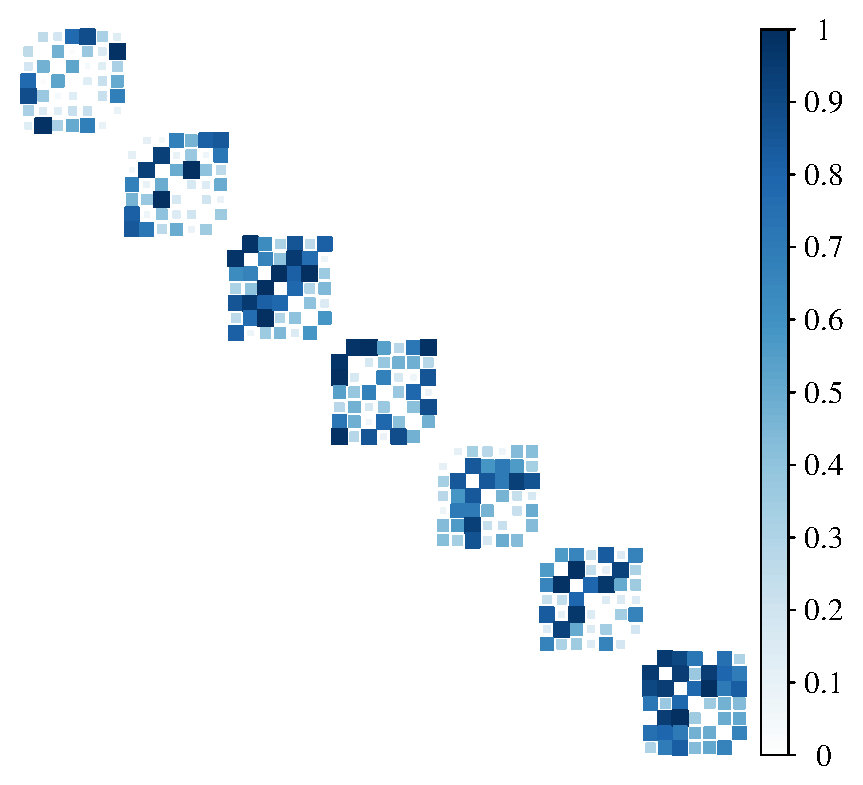
\includegraphics[width=\textwidth]{model-mismatch/latex/figures/true_mat.eps}
        \caption{Ground Truth Laplacian}
    \end{subfigure}
    ~ %add desired spacing between images, e. g. ~, \quad, \qquad, \hfill etc.
      %(or a blank line to force the subfigure onto a new line)
    \begin{subfigure}[b]{0.3\textwidth}
        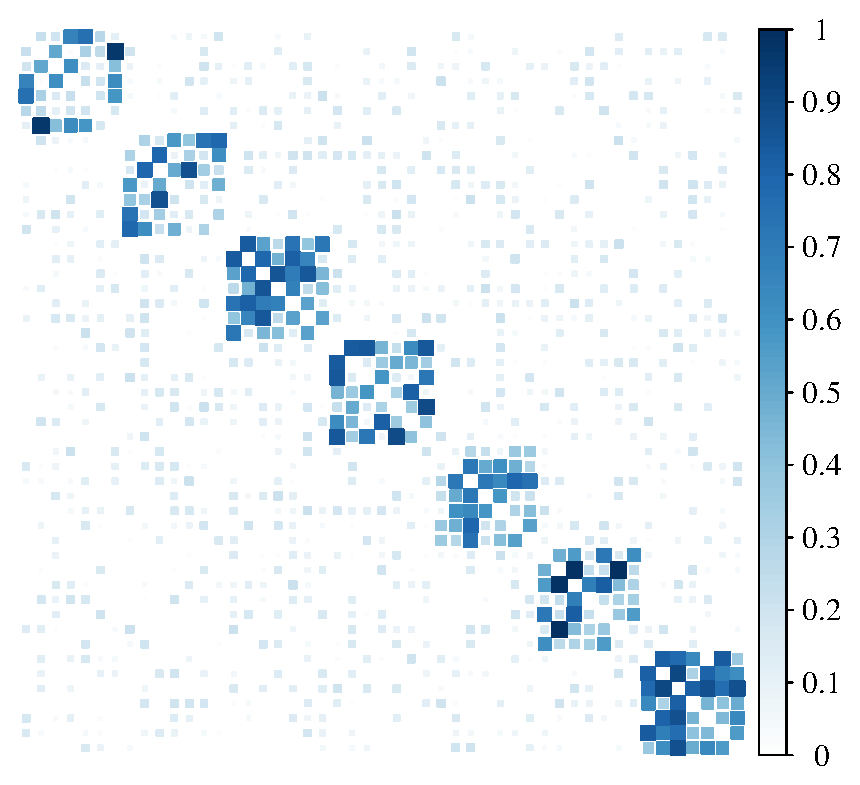
\includegraphics[width=\textwidth]{model-mismatch/latex/figures/noisy_mat.eps}
        \caption{Noisy Laplacian matrix}
    \end{subfigure}
    ~ %add desired spacing between images, e. g. ~, \quad, \qquad, \hfill etc.
    %(or a blank line to force the subfigure onto a new line)
    \begin{subfigure}[b]{0.3\textwidth}
        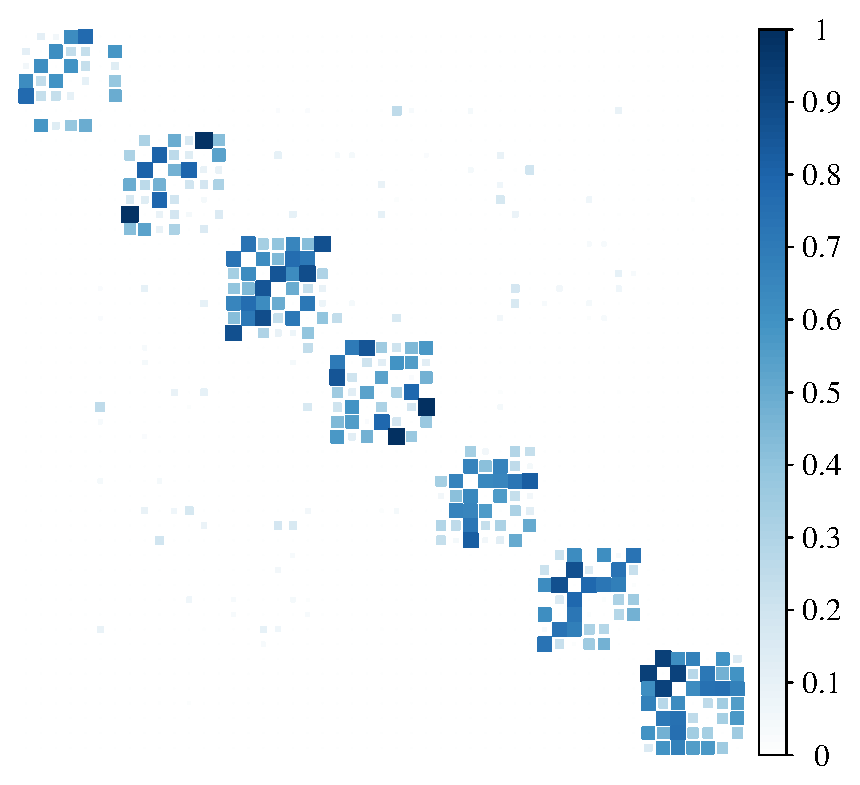
\includegraphics[width=\textwidth]{model-mismatch/latex/figures/est_mat.eps}
        \caption{Learned Laplacian ($K = 2$)}
    \end{subfigure}
        \\
    \begin{subfigure}[b]{0.3\textwidth}
        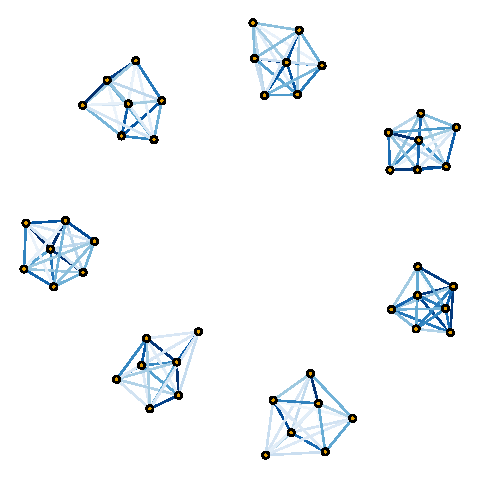
\includegraphics[width=\textwidth]{model-mismatch/latex/figures/true_graph.eps}
        \caption{Ground Truth graph}
    \end{subfigure}
    ~ %add desired spacing between images, e. g. ~, \quad, \qquad, \hfill etc.
      %(or a blank line to force the subfigure onto a new line)
    \begin{subfigure}[b]{0.3\textwidth}
        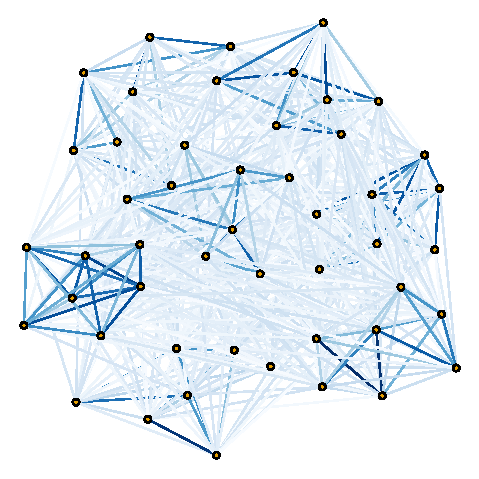
\includegraphics[width=\textwidth]{model-mismatch/latex/figures/noisy_graph.eps}
        \caption{Noisy graph}
    \end{subfigure}
    ~ %add desired spacing between images, e. g. ~, \quad, \qquad, \hfill etc.
    %(or a blank line to force the subfigure onto a new line)
    \begin{subfigure}[b]{0.3\textwidth}
        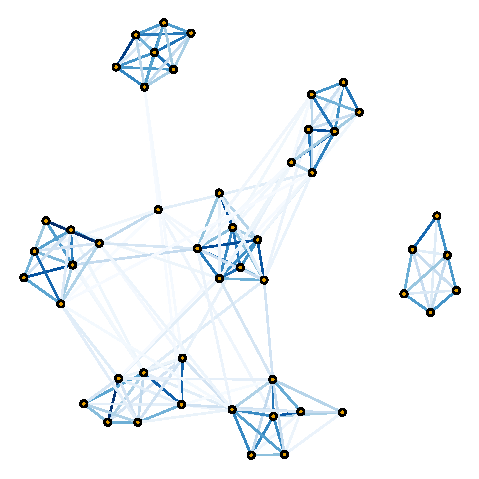
\includegraphics[width=\textwidth]{model-mismatch/latex/figures/est_graph.eps}
        \caption{Learned graph}
    \end{subfigure}
        \caption{Example of model mismatching. (a) the ground truth graph Laplacian of a seven-component graph
                 ($\mathbf{L}_{\mathsf{true}}$), (b) $\mathbf{L}_{\mathsf{true}}$ after being corrupted by noise,
                 (c) the learned graph Laplacian with a performance of
                 $(\mathsf{RE}, \mathsf{FS}) = (0.18, 0.81)$.
                 The panels (d), (e), and (f) correspond to the graphs represented by the Laplacian matrices in
                 (a), (b), and (c), respectively.}
        \label{fig:7-comp-graph}
\end{figure}

\begin{figure}[!htb]
  \centering
  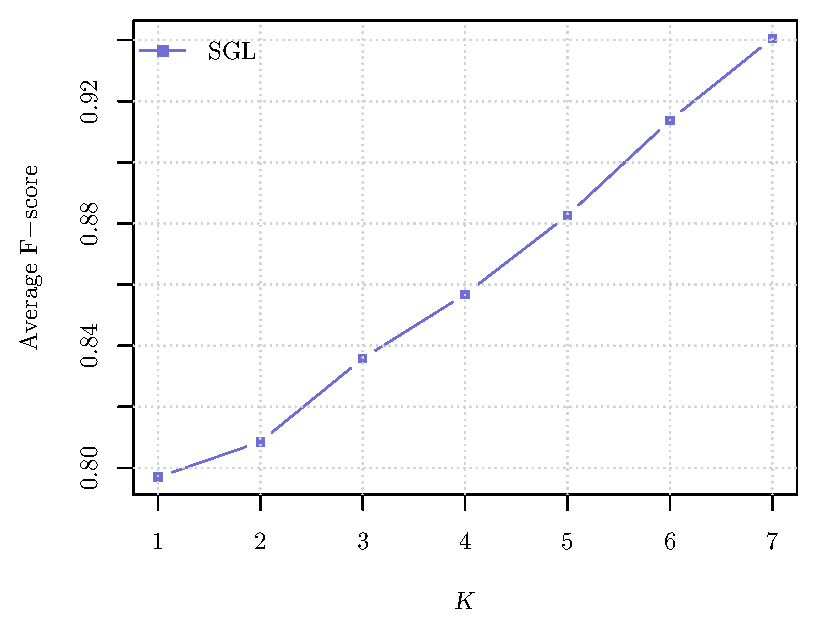
\includegraphics[width=.45\textwidth]{model-mismatch/latex/figures/fscore.eps}
  \caption{F-score as a function of the number of components $K$.}
  \label{fig:fscore-k}
\end{figure}

